\documentclass{article}
\usepackage[margin = 0.5in]{geometry}
\usepackage{amsmath, pgfplots, tkz-fct, sfmath, enumerate, multicol}
\pgfplotsset{compat = newest}
\usepgfplotslibrary{fillbetween}
\renewcommand{\familydefault}{\sfdefault}
\pagestyle{empty}
\raggedright
\everymath{\displaystyle}

\begin{document}

\subsubsection*{Area and the Definite Integral P-Set}

Using the left endpoints, approximate the area under each curve above the $x$-axis using 
\begin{enumerate}[(a)]
    \item 4 rectangles and
    \item 8 rectangles
\end{enumerate}
\begin{multicols}{3}
\begin{enumerate}
    \item $f(x) = x^2 + 2$ from $x = 0$ to 4
    \item $f(x) = x^3$ from $x = 0$ to 4
    \item $f(x) = \frac{1}{x}$ from $x = 1$ to 5
\end{enumerate}
\end{multicols}

Using the right endpoints, approximate the area under each curve above the $x$-axis using 
\begin{enumerate}[(a)]
    \item 4 rectangles and
    \item 8 rectangles
\end{enumerate}
\begin{multicols}{3}
\begin{enumerate}   \setcounter{enumi}{3}
    \item $f(x) = x^2 + 2$ from $x = 0$ to 4
    \item $f(x) = x^3$ from $x = 0$ to 4
    \item $f(x) = \frac{1}{x}$ from $x = 1$ to 5
\end{enumerate}
\end{multicols}
\vspace{10pt}

Use a graphing utility to find the area under the curve for each given interval.
\begin{multicols}{3}
\begin{enumerate}   \setcounter{enumi}{6}
    \item $\int_{0}^{4} \left(x^2 + 2\right) \, \mathrm{d}x$
    \item $\int_{0}^{4} x^3 \, \mathrm{d}x$
    \item $\int_{1}^{5} \frac{1}{x} \, \mathrm{d}x$
\end{enumerate}
\end{multicols}
\vspace{10pt}

Provide a sketch of the area under the curve for each. Then use a graphing utility to approximate the area.
\begin{multicols}{3}
\begin{enumerate}   \setcounter{enumi}{9}
    \item $\int_{1}^{6} (x^3 + 1) \, \mathrm{d}x$
    % \item $\int_{-\pi/2}^{\pi/2} \sin (x) \, \mathrm{d}x$
    \item $\int_{0}^{9}\sqrt{x} \, \mathrm{d}x$
    \item $\int_{-2}^{5} |x| \, \mathrm{d}x$
\end{enumerate}
\end{multicols}
\vspace{10pt}

% \subsubsection*{Challenge Problem}
% 13. Find the \underline{exact} area under the curve for the given piecewise function.
% \[ 
% \int_{1}^{10} f(x) \, dx \text{ if } f(x) = \begin{cases}
% 4x \quad    &\text{ if } 0 \leq x \leq 2    \\ 
% -8x+16  \quad   &\text{ if } 2 < x \leq 3    \\ 
% 8  \quad   &\text{ if } x > 3  \\ 
% \end{cases}
% \]


\newpage


\textbf{Area and the Definite Integral KEY}

\begin{multicols}{3}
\begin{enumerate}
    \item (a) $22$ \quad (b) $\frac{51}{2}$
    \item (a) 36 \quad (b) 49
    \item (a) $\frac{25}{12}$ \quad (b) $\frac{4609}{2520}$
\end{enumerate}
\end{multicols}
\vspace{10pt}
\begin{multicols}{3}
\begin{enumerate}   \setcounter{enumi}{3}
    \item (a) 38 \quad (b) 33.5
    \item (a) 100 \quad (b) 81
    \item (a) $\frac{77}{60}$ \quad (b) $\frac{3601}{2520}$
\end{enumerate}
\end{multicols}
\vspace{10pt}
\begin{multicols}{3}
\begin{enumerate}   \setcounter{enumi}{6}
    \item $\frac{88}{3} = 29.\overline{3}$
    \item 64
    \item about $1.6094$
\end{enumerate}
\end{multicols}
\vspace{10pt}
\begin{multicols}{3}
\begin{enumerate}   \setcounter{enumi}{9}
    \item 328.75
    \item 18
    \item 14.5
\end{enumerate}
\end{multicols}
\vspace{0.25in}
\begin{tabular}{p{0.3\textwidth}p{0.3\textwidth}p{0.3\textwidth}}
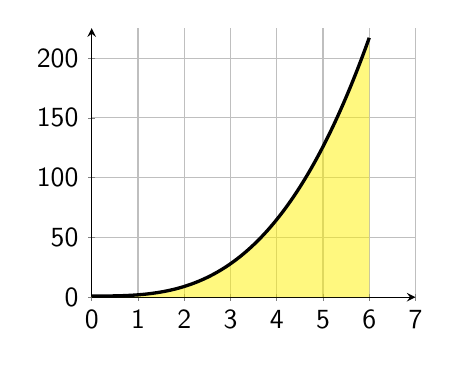
\begin{tikzpicture}[scale=0.6]
\begin{axis}
[axis lines = left, xmin = 0, xmax = 7, ymin = 0, ymax = 225, grid]
\addplot [domain = 0:6, samples=200, very thick, name path = f] {x^3+1}; 
\path[name path=axis] (axis cs:0,0) -- (axis cs:6,0);
\addplot [
        color=yellow,
        fill=yellow,
        fill opacity = 0.5
    ]
    fill between[
        of=f and axis, soft clip={domain=0:6}
    ];
\end{axis}
\end{tikzpicture}
&
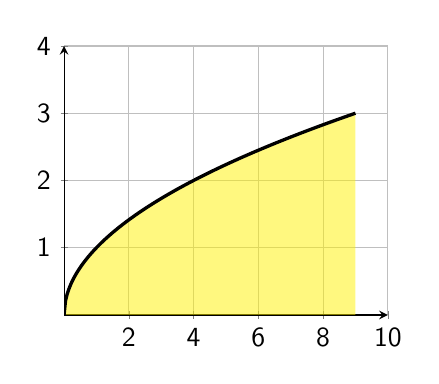
\begin{tikzpicture}[scale=0.6]
\begin{axis}
[axis lines = middle, xmin = 0, xmax = 10, ymin = 0, ymax = 4, grid]
\addplot [domain = 0:9, samples=200, very thick, name path = f] {sqrt(x)}; 
\path[name path=axis] (axis cs:0,0) -- (axis cs:9,0);
\addplot [
        color=yellow,
        fill=yellow,
        fill opacity = 0.5
    ]
    fill between[
        of=f and axis, soft clip={domain=0:9}
    ];
\end{axis}
\end{tikzpicture}
&
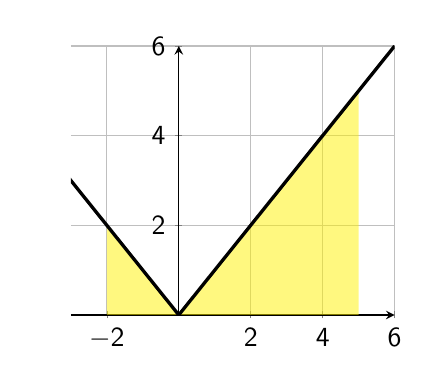
\begin{tikzpicture}[scale=0.6]
\begin{axis}
[axis lines = middle, xmin = -3, xmax = 6, ymin = 0, ymax = 6, grid]
\addplot [domain = -6:6, samples=200, very thick, name path = f] {abs(x)}; 
\path[name path=axis] (axis cs:-2,0) -- (axis cs:5,0);
\addplot [
        color=yellow,
        fill=yellow,
        fill opacity = 0.5
    ]
    fill between[
        of=f and axis, soft clip={domain=-2:5}
    ];
\end{axis}
\end{tikzpicture}
\end{tabular}

% \begin{enumerate}   \setcounter{enumi}{9}
% \item 328.75   \newline 
% \begin{tikzpicture}[scale=0.6]
% \begin{axis}
% [axis lines = left, xmin = 0, xmax = 7, ymin = 0, ymax = 225, grid]
% \addplot [domain = 0:6, samples=200, very thick, name path = f] {x^3+1}; 
% \path[name path=axis] (axis cs:0,0) -- (axis cs:6,0);
% \addplot [
%         color=yellow,
%         fill=yellow,
%         fill opacity = 0.5
%     ]
%     fill between[
%         of=f and axis, soft clip={domain=0:6}
%     ];
% \end{axis}
% \end{tikzpicture}
% \bigskip

% \item 0  \quad \newline\\
% \begin{tikzpicture}[scale=0.6]
% \begin{axis}
% [axis lines = middle, xmin = -2, xmax = 2, ymin = -2, ymax = 2, grid]
% \addplot [domain = -pi/2:pi/2, samples=200, very thick, name path = f] {sin(deg(x))}; 
% \path[name path=axis] (axis cs:-pi/2,0) -- (axis cs:pi/2,0);
% \addplot [
%         color=yellow,
%         fill=yellow,
%         fill opacity = 0.5
%     ]
%     fill between[
%         of=f and axis, soft clip={domain=-pi/2:pi/2}
%     ];
% \draw (axis cs: -pi/2,0.15) -- (axis cs: -pi/2,-0.15) node [below] {$-\frac{\pi}{2}$};
% \draw (axis cs: pi/2,0.15) -- (axis cs: pi/2,-0.15) node [below] {$\frac{\pi}{2}$};
% \end{axis}
% \end{tikzpicture}
% \bigskip

% \item 14.5   
% \begin{tikzpicture}[scale=0.6]
% \begin{axis}
% [axis lines = middle, xmin = -3, xmax = 6, ymin = 0, ymax = 6, grid]
% \addplot [domain = -6:6, samples=200, very thick, name path = f] {abs(x)}; 
% \path[name path=axis] (axis cs:-2,0) -- (axis cs:5,0);
% \addplot [
%         color=yellow,
%         fill=yellow,
%         fill opacity = 0.5
%     ]
%     fill between[
%         of=f and axis, soft clip={domain=-2:5}
%     ];
% \end{axis}
% \end{tikzpicture}
% \end{enumerate}


\end{document}


